%chktex-file 36
%chktex-file 8
%chktex-file 24
%chktex-file 35
%chktex-file 44
%chktex-file 1
\documentclass[ComputationalMathematics.tex]{subfiles}

\begin{document}

%%%%%%%%%%%%%%~~~~~~~~~~~~~~~~~~~~~~~~~~~~~~~~~~~~~~~~%%%%%%%%%%%%%%%
\section{13th of December 2018 --- F. Poloni}
%%%%%%%%%%%%%%~~~~~~~~~~~~~~~~~~~~~~~~~~~~~~~~~~~~~~~~%%%%%%%%%%%%%%%

\subsection{Lanczos algorithm}

\recap{In last lecture we saw how to factorize a matrix $A \in M(m, \R)$ with Arnoldi (i.e.~$AQ_n = Q_{n+1} \underline{H}_n = Q_n \underline{H}_n + h_{n+1, n} q_{n+1} \tr{e_1}$).}

If $A$ is \textbf{symmetric}, something special happens: $\underline{H}_n = \tr{Q}_m A Q_m$ is symmetric as well, so it is a \textbf{tridiagonal} matrix.
This improves the complexity of the Arnoldi process, because many iterations of the for loop (\texttt{j = 1~: n}) are not needed anymore, we need only two iterations.

This symmetric variant of Arnoldi is called \emph{Lanczos algorithm}, and such algorithm reduces the cost to $n$ matrix products + $O(mn)$.

Suppose $A=A^T$ is positive definite.
Then, we can find the solution to $Ax=b$ by minimizing the (strictly convex) function $f(x) = \frac{1}{2} \tr{x}Ax - \tr{b}x$. 

Surprisingly, conjugate gradient on this problem can be interpreted as a Krylov subspace method.

The pseudocode of such algorithm can be found in \Cref{alg:7dic_ConjGrad}, where $x_k$ is the current iterate, $r_k = b-Ax_k = -\nabla f(x_k)$ is the residual and $d_k$ is the search direction.

\algo{alg:7dic_ConjGrad}{Pseudocode for the conjugate gradient method.}{
  \Procedure{CG_iteration}{}
    \State~$x_0 \gets 0$;
    \State~$r_0 \gets b$;
    \State~$d_0 \gets b$;
    \For{k = 1:n}
      \State~$\alpha_k \gets (\tr{r_{k-1}} r_{k-1}) / (\tr{d_{k-1}} A d_{k-1})$;
      \State~$x_k \gets x_{k-1} + \alpha_k d_{k-1}$;
      \State~$r_k \gets r_{k-1} - \alpha_k A d_{k-1}$;
      \State~$\beta_k \gets (\tr{r_k} r_k) / (\tr{r_{k-1}} r_{k-1})$;
      \State~$d_k \gets r_k + \beta_k d_{k-1}$;
    \EndFor%
  \EndProcedure%
}

Notice that the search direction (line $10$) is modified adding a multiple of the previous search direction to the residual and $\beta_k$ is chosen such that $d_k$ and $d_{k-1}$ are A-orthogonal (formally, $\tr{d_k}Ad_{k-1} = 0$). 

Conversely, the next point is chosen in order to minimize the objective function $f(x_{k-1} \alpha_k d_{k-1})$.

As far as the complexity is concerned, the space complexity is constant (three vectors) and the time complexity is O(mn).

\begin{theorem}
  $K_k(A, b) = span(x_1, x_2, \ldots, x_k) = span(d_0, d_1, \ldots, d_{k-1}) = span(r_0, r_1, \ldots, r_{k-1})$.
\end{theorem}

\begin{theorem}
The residuals are orthogonal and the search directions are $A$-orthogonal.
Formally,
  $\tr{r_j} r_k = \tr{d_i} A d_k = 0,~\forall~i<k$.
\end{theorem}

\begin{proof}
By induction:
  Let us assume we proved the thesis $\tr{r_j} r_k = 0$ for $k-1, k-2, \ldots, 0$.
  Since $x_k = x_{k-1} \alpha_{k} d_{k-1}$, the residual $r_k = b-Ax_k = b - A(x_{k-1} + \alpha_{k} d_{k-1}) = b - A x_{k-1} - \alpha_k A d_{k-1} = r_{k-1} - \alpha_k A d_{k-1}$.

  Let us compute $\tr{r_j} r_k = \tr{r_j} (r_{k-1} - \alpha_k A d_{k-1})$.
  \begin{itemize}
    \item If $i < k-1$ then $\tr{r_j} r_{k-1} - \tr{r_j} \alpha_k A d_{k-1} = 0$, because the first term is $0$ from induction hypothesis and $\tr{r_j} \alpha_k A d_{k-1} = 0$, because $r_j \in K_{k-1}(A, b) = span(d_0, d_1, \ldots, d_{k-2})$.
    \item If $i = k-1$, $0 = \tr{r_{k-1}} (r_{k-1} - \alpha_k A d_{k-1}) = \tr{r_{k-1}} r_{k-1} - \alpha_k \tr{r_{k-1}} A d_{k-1}$ holds if $\alpha_k=\frac{r_{k-1}^T r_{k-1}}{r_{k-1}^T A d_{k-1}}$. 
      We are left with proving that $\alpha_k=\frac{r_{k-1}^T r_{k-1}}{r_{k-1}^T A d_{k-1}} = \alpha_k=\frac{r_{k-1}^T r_{k-1}}{d_{k-1}^T A d_{k-1}}$.

      This is true, since $d_{k-1} = r_{k-1} + \beta_{k-1} d_{k-2}$, so $\tr{d_{k-1}} A d_{k-1} = \tr{(r_{k-1} + \beta_{k-1} d_{k-2})} A d_{k-1} = \tr{r_{k-1}} A d_{k-1} + \beta_{k-1} \tr{d_{k-2}Ad_{k-1}}$ and the second part is equal to $0$ by induction. 
  \end{itemize}
\end{proof}

Notice that this base is not orthonormal, we need to rescale it to obtain an orthonormal one, moreover, $\frac{1}{\norm{r_i}}r_i$ coincides (up to a sign) with the $q_i$ obtained with Arnoldi.

We are left with writing the equation we need to solve at each iteration, namely we need to ensure that $r_k = b - A x_k$ is orthogonal to all vectors of $K_k(A, b)$ which is equivalent to requiring $\tr{Q_k} (b - Ax_k) = 0$ or, equivalently, $\norm{b} e_1 = H_k y_k$.

In figure \Cref{fig:13dic_parallel} we can see a comparison between Arnoldi algorithm and the conjugate gradient.

\begin{figure}[h]
  \centering
  \subfloat[][Arnoldi]{\includegraphics[width=0.35\textwidth]{pics/13dic/1.png}\label{subfloat:13dic_arnoldi}}
  \hspace{0.5cm}
  \subfloat[][Conjugate gradient]{\includegraphics[width=0.35\textwidth]{pics/13dic/2.png}\label{subfloat:13dic_cg}}\\
  \caption{Traditional orthogonality (Arnoldi) leads to the minimization of the 2-norm, while in the conjugate gradient we impose A-orthogonality and we get a good approximation in several norms.}\label{fig:13dic_parallel}
\end{figure}

As far as convergence speed is concerned, 

\begin{theorem}
  $x_k$ is the best approximation of the exact (and unknown) solution $x$ to $Ax=b$ in $K_k(A, b)$ in the $A$-norm, i.e. $x_k = arg \min\limits_{z \in K_k(A, b)} \tr{(x-z)} A (x-z)$
\end{theorem}

\begin{theorem}
Let $\lambda_{\max}$, $\lambda_{\min}$ be the maximum/minimum eigenvalue of $A$; then, CG converges with rate:
\[
  \norm{x-x_k} \leq {\left( \frac{\sqrt{\lambda_{\max}} - \sqrt{\lambda_{\min}}}{\sqrt{\lambda_{\max}} + \sqrt{\lambda_{\min}}}\right)}^k \norm{x-x_0}
\]
\end{theorem}

We can rewrite it in terms of a more familiar quantity: for a positive definite matrix, eigenvalues and singular values coincide, hence:
\[
\frac{\sqrt{\lambda_{\max}} - \sqrt{\lambda_{\min}}}{\sqrt{\lambda_{\max}} + \sqrt{\lambda_{\min}}} = \frac{\sqrt{\sigma_1} - \sqrt{\sigma_m}}{\sqrt{\sigma_1} + \sqrt{\sigma_m}} = \frac{\sqrt{\frac{\sigma_1}{\sigma_m}}-1}{\sqrt{\frac{\sigma_1}{\sigma_m}}+1} = \frac{\sqrt{\kappa(A)}-1}{\sqrt{\kappa(A)}+1}.
\]
For large values of $\kappa(A)$, this is approximately $1 - \frac{2}{\sqrt{\kappa(A)}}$, while if $\kappa(A) \approx 1$ the convergence speed is very high.

As for GMRES, if $A$ has only $n$ different eigenvalues, then this minimum reaches $0$ after $n$ steps. If the eigenvalues of $A$ are `clustered', one can construct polynomials such that $q(\lambda)$ is small for each $\lambda$ then fast convergence is implied.

\end{document}
